\chapter{网络功能虚拟化相关技术}
\label{chap:relatedwork}

\section{网络功能虚拟化发展概况}
2012年10月,ETSI的NFV规范小组在德国的达姆施塔特发表了关于软件定义网络(SDN, Software Defined Network)和OpenFlow的白皮书,期间正式推出了NFV概念。自白皮书发表以来,该小组制定了每两年为一个发布周期的工作计划,持续推出更加具体的协议规范和标准术语定义以及NFV的使用案例。截止本文,NFV小组已经进入了第三个发布周期。

在第一个周期2013-2014年内,小组的主要工作目标是:
\begin{enumerate*}[label=\itshape\alph*)\upshape]
	\item 推动网络运营商融合NFV。
	\item 将已有的适用标准纳入网络服务和产品中。
	\item 以促进创新和培育供应商开放的生态系统为目标,同步地开发新的技术规范。
\end{enumerate*}
截止2014年,工作组除了前期发布的6篇定义性文档,又陆续发布了11篇详细的技术规范,包括。。。 第一套文档标志着NFV的标准化初期工作已经完成,需要对划分的各个工作领域进行进一步的详细定义和约束。

第二个周期2015-2016年,小组的工作重心已经转移到了VIM,VNFM,NFVO以及各功能接口的具体定义中。进一步的,在该阶段的工作中,小组还重点推出了适用于当前NFV服务需求的信息模型参考,在模型中预留了解决各项实际问题的参数接口,为各厂商开发自己的NFV服务框架提供指导。各项文档均已在ETSI官方网站发布。

目前,NFV规范小组正处在2017-2018发布周期内。根据已发布的计划,在本周期内他们有23个工作目标,包括20个新功能点和3个对上一周期的已发布文档的补充。在该周期内,小组的工作重点是深入定义核心的NFV信息模型,完善支持NFV非业务子系统接口如计费,账单,用户管理,监管,安全等,以及对MANO服务的多方面支持。同时在近些年来,NFV工作组联合了如Linux Foundation,OpenDayLight等开源社区以及工业界各服务提供厂商,旨在携手推进NFV落地实现,与现有业务平台平滑过渡衔接。他们推出了各种开源的NFV平台如OPNFV,OpenSource MANO,Open-O, Cloudify等等。学术界近年来对NFV的研究也进行得如火如荼,相关介绍在第 \ref{chap:Introduction} 章节中已有详细的介绍。


\section{常见的网络I/O虚拟化技术}
虚拟化技术作为NFV的基础,是实现NFV的关键技术。I/O虚拟化,特别是网络I/O虚拟化,更是直接影响了NFV性能的关键因素。在本节中,我们将介绍和分析三种主流的网络虚拟化模型:设备仿真模型(Device Emulation),分离驱动程序模型(Split-driver)和硬件辅助模型(Hardware-assisted),并对这三种模型在实际应用场景下做出对比。

\subsection{设备模拟模式}
设备模拟模式是一种通过在虚拟机监视器中模拟敏感指令和特权指令的方式来模拟物理设备I/O操作的全虚拟化实现方式。如图 \ref{fig:device_emu} 所示。这种模式充分利用二进制翻译技术和直接执行技术的组合来从客户操作系统中抽象和分离底层硬件,实现纯软件方式的硬件仿真。虚拟机操作系统实例和用户级别指令可以在没有感知底层虚拟化环境的情况下不加修改地运行,所以设备模拟模式为I/O操作提供了最佳性能隔离和安全性,简化了客户端虚拟机的迁移操作和提升了其可移植性。工业界有很多成熟的产品如VMware Workstation \cite{sugerman2001virtualizing} 和VMware ESX Server \cite{ahmad2003analysis} 都支持这种I/O虚拟化的方式。此外,XEN和KVM的QEMU也可以配置支持设备模拟模式的I/O虚拟化。
\begin{figure}[!htp]
	\centering
	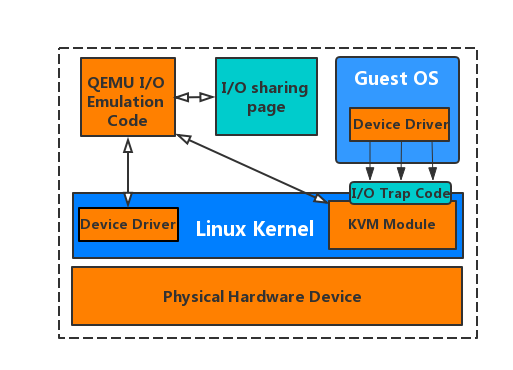
\includegraphics[width=0.8\textwidth]{Device_Emulation.png}
	\bicaption[fig:device_emu]{设备模拟模式示意图}{设备模拟模式示意图}{Fig}{Device Emulation}
\end{figure}
但是,这种方法也存在很大的缺陷,由于虚拟机监视器需要动态翻译所有操作系统指令并缓存所有结果,因此虚拟机监视器设备驱动程序一旦发生故障将导致所有客户虚拟机的I/O中断。而且,由于在运行时对这些敏感和特权的指令请求处理需要进行代价高昂的陷入和仿真操作,频繁的此类操作将引起巨大的性能开销,成为影响I/O性能的瓶颈。根据已有的研究,每个I/O操作的陷入和仿真都将导致客户操作系统和虚拟机监视器之间的上下文切换,其成本约为 3000~5000 个CPU周期 \citen{dong2011optimizing} 。根据已有的研究实验显示,这样的开销显着地降低了近10倍的I/O吞吐量。这一性能瓶颈挑战严重阻碍了将设备仿真方法部署到高性能网络和配备现代高性能网卡(例如40/100 Gbps 网卡)的数据中心中。NFV的应用场景下需要数量众多的虚拟机频繁的使用各自的网络I/O设备,设备模拟的方式并不能胜任该场景下对I/O设备高性能的需求。

\subsection{分离驱动模式}
为了缓解虚拟机监视器参与模拟的高昂开销,Xen团队首先在半虚拟化场景下开发了分离驱动模式(Split-Driver) \cite{barham2003xen} 。紧随其后,KVM的virtio \cite{russell2008virtio,kivity2007kvm} ,VMware tool和VM interface \cite{amsden2006vmi} 也支持了在半虚拟化的分离驱动模式。本文以virtio为例,介绍在KVM平台下奋力驱动模式的实现原理。KVM的分离驱动模型如图 \ref{fig:split_dri} 所示,它由主机中的前端virtio驱动和后端驱动组成。当虚拟机向服务器内的另一台虚拟机发送数据时,虚拟机首先将数据加载到其vring缓冲区中的队列,并修改其描述符表。随后通知KVM产生vm-exit信号,并使用ioeventfd方法允许vHost驱动程序接收来自客户端虚拟机的信号。
\begin{figure}[!htp]
	\centering
	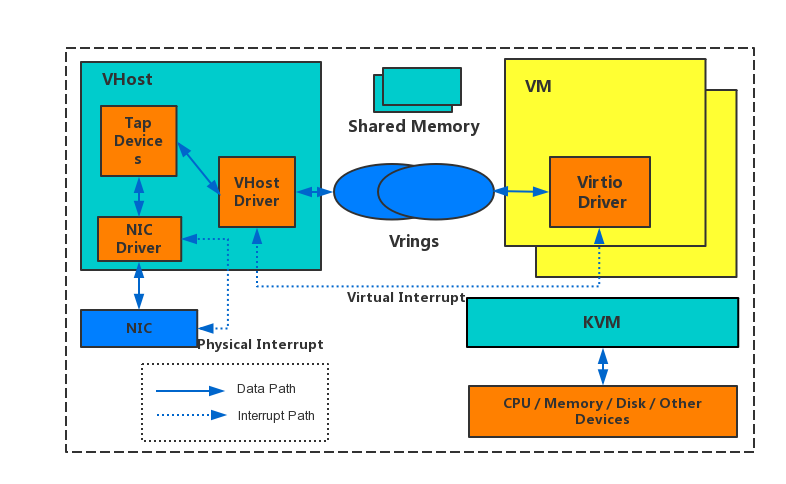
\includegraphics[width=0.8\textwidth]{Split_driver.png}
	\bicaption[fig:split_dri]{Split-driver模式示意图}{Split-driver模式示意图}{Fig}{Split-driver Model}
\end{figure}
当vHost驱动获得信号后,前端程序将获取有效队列的物理地址,并将需要传输的数据复制到绑定tap设备地址空间。数据通过网络协议栈被传送到目的地址上。在传送过程中,前端驱动发现如果目标地址是同一台机器上的虚拟机,vHost将利用零拷贝机制,通过共享内存直接将数据的地址指针发送到到目标虚拟机的对应驱动中。当目标虚拟机收到数据后会触发一个回调信号函数,并让虚拟机将传输的数据拷贝放入自己的vring读取队列。总而言之,在分离驱动模式下的虚拟机之间的数据传输可以被看作是将数据从一个内存区域复制到另一块存储区域。分离驱动模式采用高效的I/O通信通道 (I/O Channel) 来避免虚拟机监视器对模拟端口I/O和内存映射功能的干预。因此,分离驱动模式可以利用同样的物理资源达到比设备仿真模式下更高的吞吐量同时降低CPU的利用率。即使半虚拟化方式需要对操作系统内核进行深度修改,无法做到像全虚拟化方式那样对不同客户机操作系统广泛的支持,分离驱动模式还是显示出了其在虚拟机管理和虚拟机迁移方面的巨大灵活性,在当下的虚拟机监视器和虚拟机操作系统中得到了广泛的支持。


\subsection{硬件辅助模式}
设备仿真和分离驱动模式都被分类为基于软件的I/O虚拟化,这种基于软件的模式实现了丰富的I/O设备功能同时简化了对虚拟机I/O设备的管理。然而,这种方式也并不是完美无缺的,纯软件实现方式在面对大量的陷入-仿真操作或者大块数据拷贝的时候会面临高昂的系统开销,这个时候我们可以借助硬件辅助的模式来解决我们的瓶颈。硬件辅助I/O虚拟化模式是为共享本地设备而开发的,它通过继承I/O内存管理单元 (IOMMU) 的用户权限来使用直接I/O技术从而实现绕开虚拟化的内存保护和地址转换,为虚拟机直接分配真实的I/O设备。PCI-SIG工作组针对这种I/O虚拟化的方式制定了规范,通过为每个虚拟机提供独立的内存空间,中断和DMA流来绕过虚拟机监视器直接参与数据处理。特别的,PCI-SIG推出了单根I/O虚拟化 (SR-IOV) 技术,这项技术为针对PCIe设备设计了一组硬件增加技术,通过去除虚拟机监视器在数据包分类和内存地址翻译的干预来实现基于专门硬件的增强。
\begin{figure}[!htp]
	\centering
	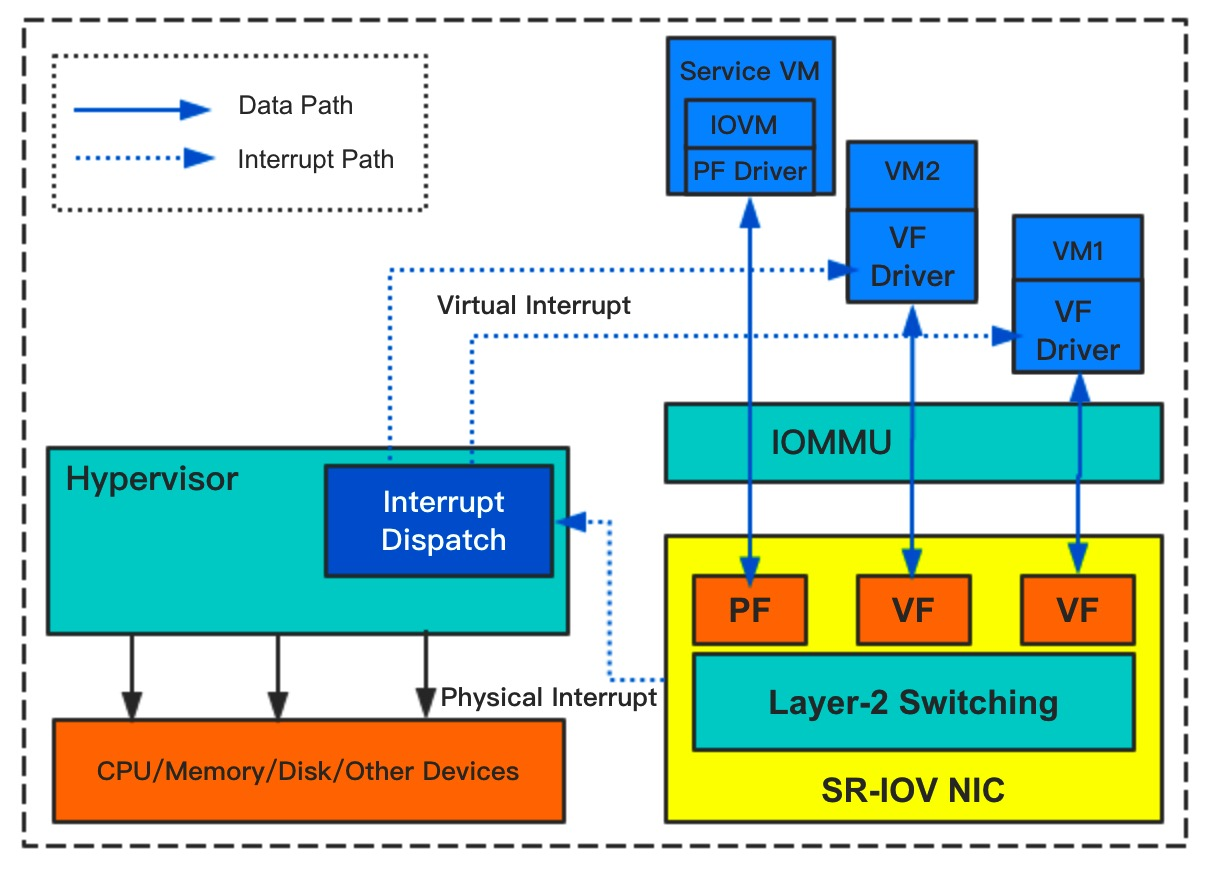
\includegraphics[width=0.8\textwidth]{SR_IOV.jpg}
	\bicaption[fig:hardware_ass]{硬件辅助模式示意图}{硬件辅助模式示意图}{Fig}{Hardware-assisted Model}
\end{figure}
SR-IOV虚拟化模式结构如图 \ref{fig:hardware_ass} 所示,一个支持SR-IOV功能的设备可以由虚拟机监视器分配多个虚拟设备(VF, Virtual Function),以普通PCI设备的身份被分配PCI地址空间。宿主机中的物理设备 (PF, Physical Function) 的驱动程序负责管理和配置VF,而在被分配VF的虚拟机操作系统中,驱动程序将其当做普通的直接分配的物理设备来使用,通过IOMMU直接访问自己专有的VF。通过这样的方式,SR-IOV可以绕过虚拟机监视器实现数据的传递,从而减少移动数据的开销,在降低CPU利用率的同时,减少系统的延迟并挺高网络吞吐量。但是需要指出的是,这种硬件辅助的方式需要手动进行虚拟网络功能的配置,无法实现像软件实现方式那样灵活的迁移和扩展。并且一块PF所能分配的VF是有上限的,这也从硬件角度限制了硬件辅助方式的在多虚拟机应用场景下的应用。


\section{非一致性存储访问架构}
众所周知,NFV的目标是在大容量的标准通用服务器上运行传统通信业务,而现在通用的标准服务器基本都是遵循非一致性存储访问架构 (NUMA, Non-Uniform Memory Access) 的服务器阵列,为了更好地完成NFV到通用服务器上的迁移,了解通用服务器的基础架构十分必要。图 \ref{fig:numa} 所示的是Intel Haswell架构下多核处理器示意图,在NUMA服务器中每个处理节点 (Socket/Die) 与通过内存访问控制器 (MC,Memory Controller) 与相邻的内存直接相连。同一个处理节点中的多个物理核拥有自己独占的L1/L2级缓存并且通过节点内部链路通道共享L3缓存,内存访问控制器以及PCI-e接口。在一个处理节点内部的的数据传输是通过点对点的高速数据通路 (例如Intel的QPI) 传输的。除了同一个节点内通信,不同的节点间也由相同的高速数据通路相连,不同的处理器节点要访问别的节点的内存时,需要通过内存控制器进行远程访问。
\begin{figure}[!htp]
	\centering
	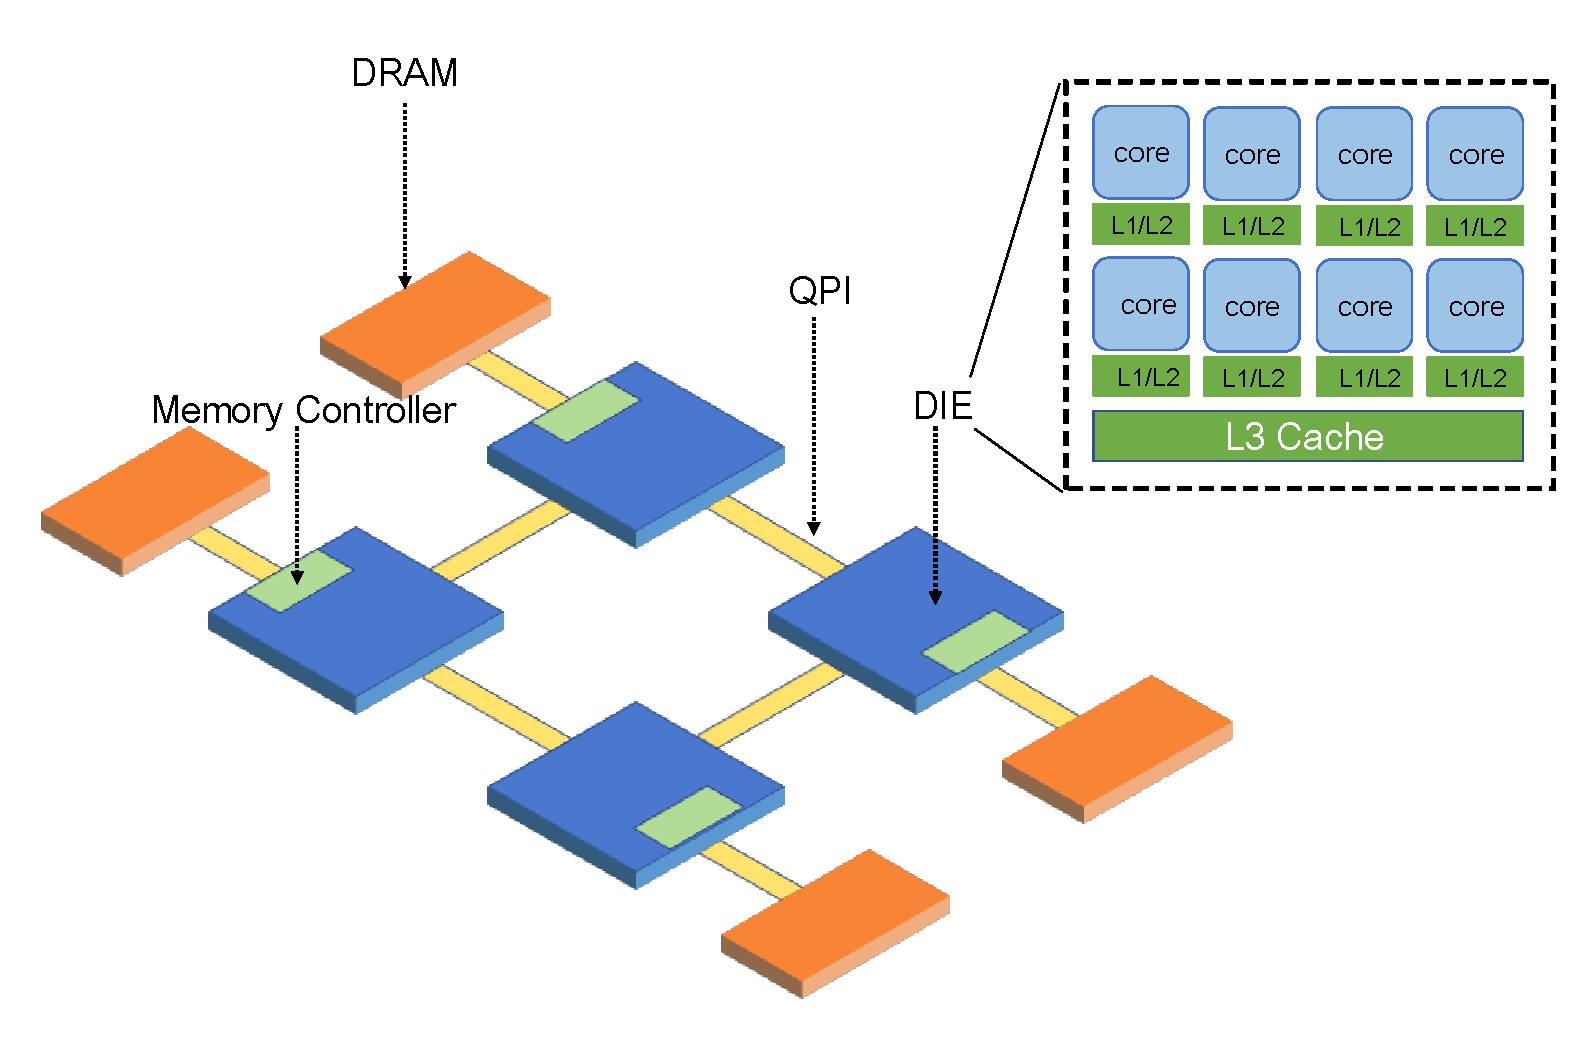
\includegraphics[width=0.8\textwidth]{numa.pdf}
	\bicaption[fig:numa]{Intel Haswell架构非一致性存储访问示意图}{Intel Haswell架构非一致性存储访问示意图}{Fig}{NUMA Architecture}
\end{figure}
在NUMA架构下,本地和远程内存访问由于机制的差异存在性能上的差异,而节点内共享的内存控制器在竞争过高的情况下也容易成为性能瓶颈导致内存访问性能的剧烈下降,所以如何针对多核通用服务器下非一致性访问的特性来优化应用一直是学术界所面对的经典挑战之一。NFV应用迁移到多核服务器中,不可避免地会遇到NUMA架构所带来的问题,而SFC的服务组织形式下同一条服务链上的虚拟机彼此之间存在大量的数据拷贝传输,如何处理好基于物理架构的物理资源对实现高性能的NFV具有重要意义。
\begin{figure}[!htp]
	\centering
	\subfigure[Netperf带宽测试]{
		\label{exp:netperf_bandwidth}
		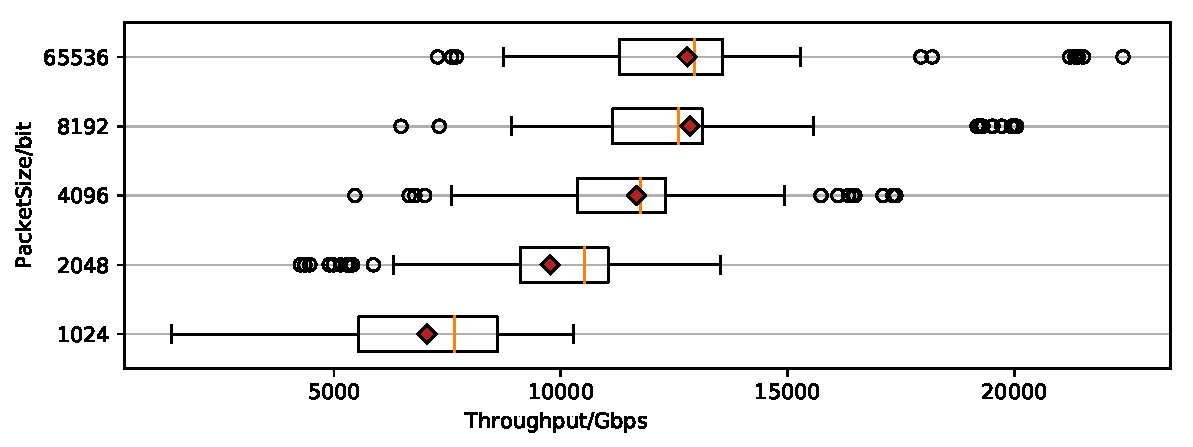
\includegraphics[width=0.8\textwidth]{observation/box1.pdf}
	}
	\subfigure[Httperf带宽测试]{
		\label{exp:httperf}
		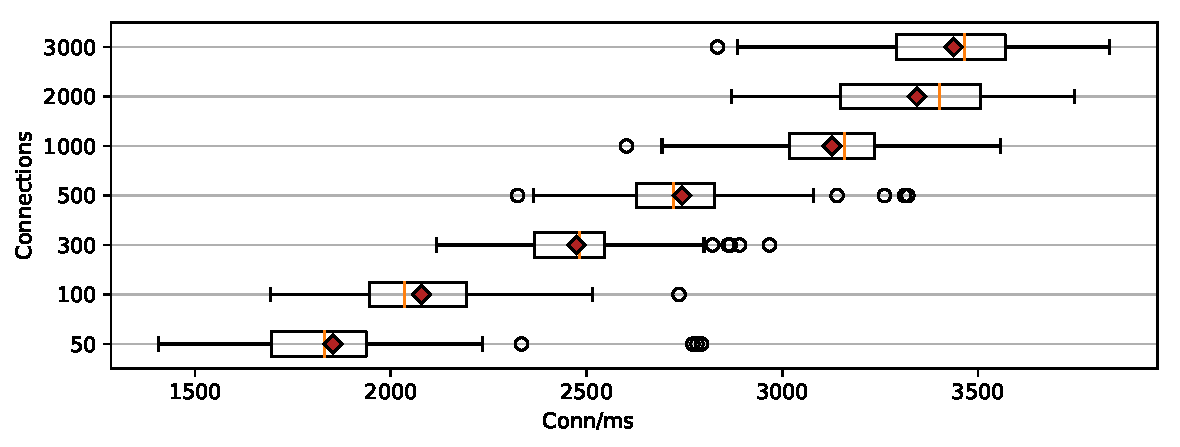
\includegraphics[width=0.8\textwidth]{observation/box2.pdf}
	}
	\subfigure[Netperf延迟测试]{
		\label{exp:netperf_latency}
		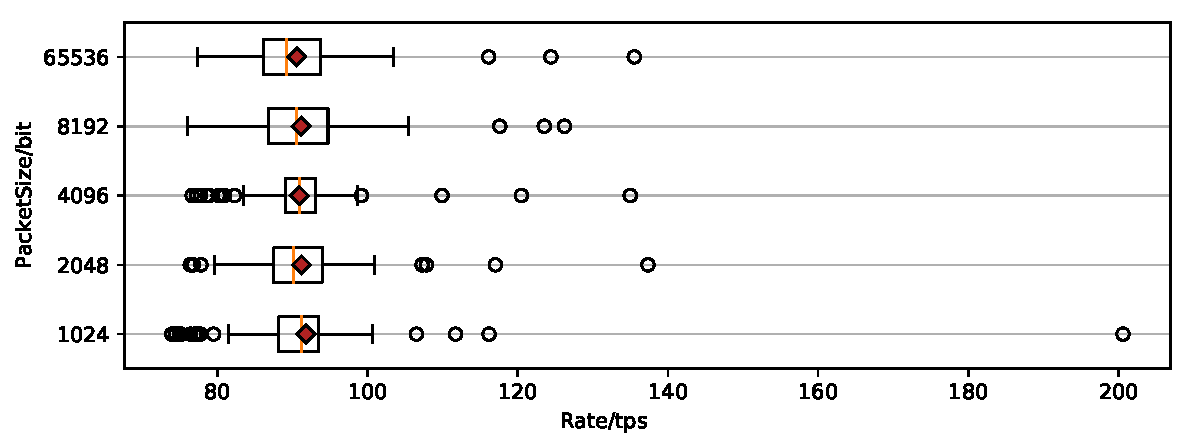
\includegraphics[width=0.8\textwidth]{observation/box3.pdf}
	}
	\bicaption[exp:observe]{模拟应用性能观测结果}{模拟应用性能观测结果}{Fig}{Application Performance Observation}
\end{figure}
\section{多核物理机性能观测与分析}
\label{related:observe}

在多核物理机中,由于存在非一致性存储访问架构的影响,传统应用都针对了NUMA问题进行了对应的优化,如经典的NUMA-aware的线程调度器numad\footnote{https://access.redhat.com/documentation/en-us/red\_hat\_enterprise\_linux/7/html/performance\_tuning\_guide/sect-red\_hat\_enterprise\_linux-performance\_tuning\_guide-tool\_reference-numad}以及已经集成进Linux内核的Auto-NUMA-Balancing机制\footnote{www.redhat.com/files/summit/2014/summit2014\_riel\_chegu\_w\_0340\_automatic\_numa\_balancing.pdf}。在NFV应用的场景下,网络功能单元是以虚拟机的形式存在,节点间的数据传输实质上是虚拟机利用网络虚拟化的技术进行通信。从服务器硬件的角度看,可以当做一个虚拟机线程向另一个虚拟机线程拷贝或者接收数据。那么在这样的前提下,虚拟机线程所分配的物理资源之间的亲和度关系对虚拟机线程间通信的性能就造成影响。为了验证这一想法,我们在一台通用服务器上进行了模拟NFV应用的的测试。测试平台具体参数见实验部分的表 \ref{tab:configure} ,使用的虚拟化平台为KVM,网络虚拟化方式为virtio。我们选取了Netperf和Httperf两个基准测试工具,分别模拟微观的数据包负载和宏观的应用负载下来测试性能表现。实验使用两台虚拟机,其中一台固定在一个处理器节点上并绑定本地内存作为虚拟机的分配内存,而另一台虚拟机则不断更改所绑定的物理核及内存,以所有绑定情况作为测试样本,测试的结果如图
 \ref{exp:observe} 所示。

我们使用盒图的方式来展现模拟应用性能测试观测结果,分别观测了微观下数据包带宽和延迟以及宏观下网络应用应用的测试结果。根据观测不难发现,在分配了相同的物理资源下,不同的资源亲和度情况下性能结果分布的离散程度很高,数据盒的宽度较大并且有大量的离群点出现,离群点之间的观测值差异甚至达到了接近三倍的差距如图 \ref{exp:netperf_bandwidth} 所示。根据这样的测试结果,我们认为针对虚拟机物理资源间的亲和度来优化服务链中的资源分配是十分必要的。

\section{Clearwater平台介绍}
\label{intro:clearwater}
目前全球的运营开发商都在加速商用的VoLTE开发,多媒体子系统 (IMS)是4G VoLTE商用组件之一,因此也引起了工业界格外的重视。NFV兴起以来,工业界纷纷在尝试将IMS系统部署在NFV平台环境中,探索IMS应用场景在NFV生产环境中的实现,希望能够利用虚拟机技术加速电信业务的研发和部署,降低业务升级的成本和周期。根据我们的调研,在开源的IMS系统领域,有两个十分知名的项目:Clearwater\footnote{项目由Metaswitch Networks 提供赞助,官方网址为 http://www.projectclearwater.org/ }与Kamalio\footnote{https://www.kamailio.org/w/}。而在这两者之中,ClearWater系统更是因为其为云计算平台量身打造的多媒体子系统定位而广受众多厂商和研发人员的欢迎,开发社区十分火热,产品也在迅速的迭代中。它采用大型互联网软件架构的设计思路,以微服务的方式设计各个组件,使得系统本身具有很好的伸缩能力,成为了一个电信级别的开源IMS系统。
其分布式版本的系统架构图如图 \ref{fig:clearwater} 所示,可以看出该系统主要有三个核心的组件,Sprout,Dime,Vellum和其他边缘组件组成。其中,Sprout节点作为注册和权限管理的路由代理,主要负责处理客户端的认证和应用服务器ISC接口的通信。Sprout节点还包含内置的MMTEL应用服务器,在运行过程中Sprout不负责存储任何持久化的数据,而是通过http协议到Homestead和homer服务中读取HSS的配置信息,如用户信息和MMTEL服务配置等;通过远程调用接口从Vellum中获取用户的注册信息和当前状态等。Dime节点主要负责运行Homestead和Ralf服务,包括对HSS信心的缓存等。而Vellum服务则负责存储各种持久化信息,包括用户的注册注册信息,当前服务的始终状态以及各种权限和密钥等。
\begin{figure}[!htp]
	\centering
	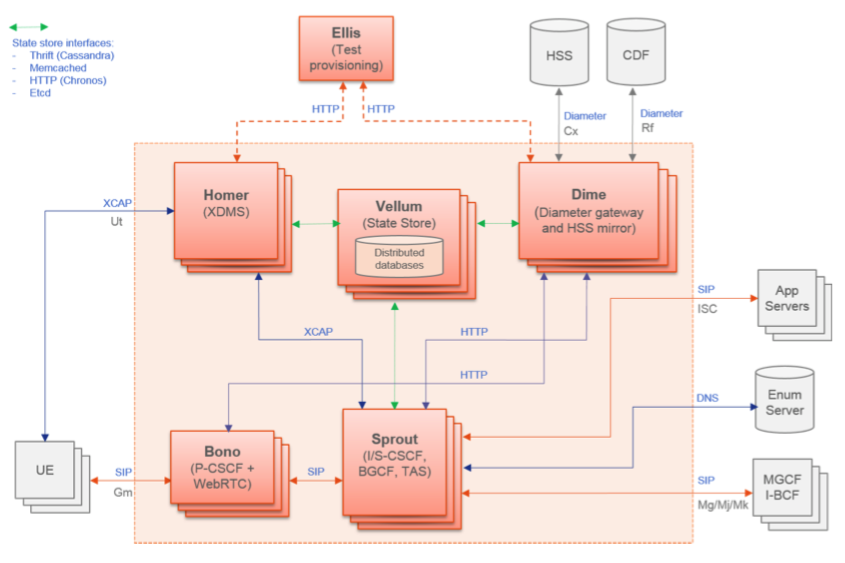
\includegraphics[width=1.0\textwidth]{clearwater/clearwater_arch.png}
	\bicaption[fig:clearwater]{Clearwater系统架构图}{Clearwater系统架构图}{Fig}{Clearwater Architecture}
\end{figure}
Clearwater是针对云计算数据中心开发的IMS系统。众多大型电信运营商纷纷采用基于IMS的标准架构作为其IP语音通话、视频和消息服务的基础构建,用以取代基于传统电路交换系统的上一代VoIP业务系统。Clearwater遵循IMS架构原则,实现了IMS核心网络所需的所有关键标准化接口。有别于别的IMS实现,Clearwater是从云计算作为基础设施的角度设计的。通过结合已在许多全球Web应用程序中验证过的设计模式和开源软件组件,Clearwater实现了前所未有的大规模可扩展性和卓越的成本效益的组合。

\section{本章小结}
本章主要介绍了与网络功能虚拟化技术已经本课题相关的一些技术背景。首先,本章简单总结了下网络功能虚拟化的发展历史和当前的发展现状,介绍了网络功能虚拟化出现的背景,包括与网络功能虚拟户实现相关的虚拟化技术以及多核服务器的架构背景。通过多核服务器的性能观测实验说明了网络功能虚拟化在多核服务器中实现索要面临的实际问题。最后本章着重介绍了本研究所基于NFV实际应用平台Clearwater,包括其业务功能简介和基本架构介绍。